\begin{figure*}[ht!]
    \centering
    \begin{subfigure}[t]{0.9\linewidth}
        \centering
        
\includegraphics[width=0.9\linewidth]{figures/evaluation/SLO_legend_MFS.pdf}
    \end{subfigure}
    \vspace{-0.5em}
    \begin{subfigure}[b]{0.24\linewidth}
        \centering
        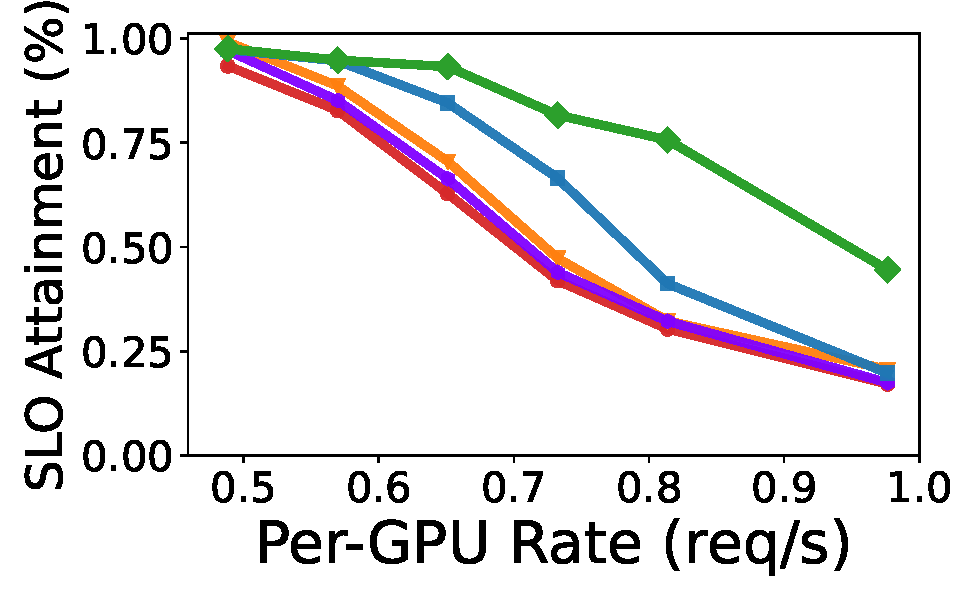
\includegraphics[width=\linewidth]{figures/evaluation/sim_qwenA/qwenA_mixtral8x22B_bw200.pdf}
        \caption{Mixtral-8x22B}
        \label{fig:evaluation:qwenA:mixtral_200}
    \end{subfigure}
    \hfill
    \begin{subfigure}[b]{0.24\linewidth}
        \centering
        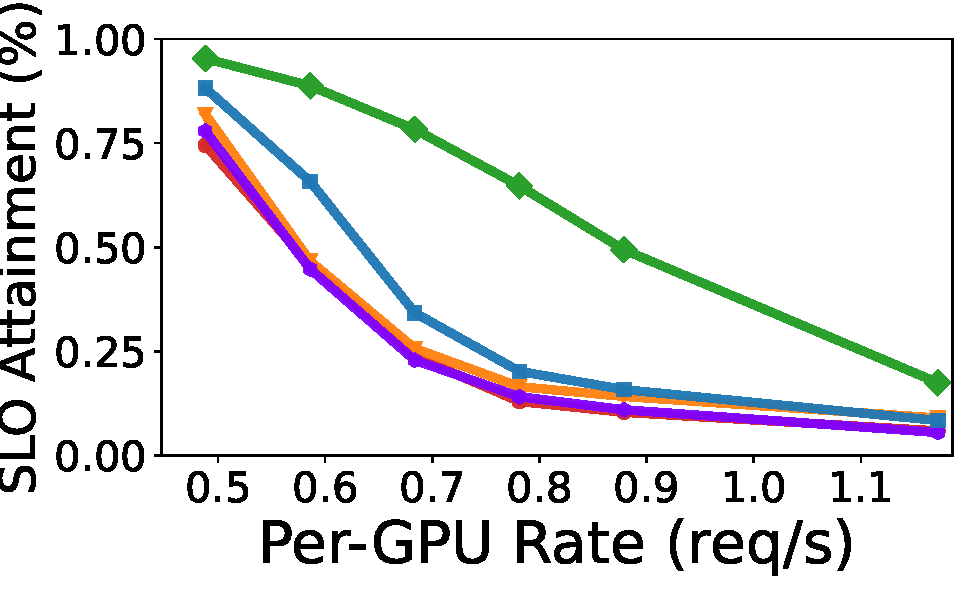
\includegraphics[width=\linewidth]{figures/evaluation/sim_qwenA/qwenA_dbrx_bw200.pdf}
        \caption{DBRX}
        \label{fig:evaluation:qwenA:dbrx_200}
    \end{subfigure}
    \hfill
    \begin{subfigure}[b]{0.24\linewidth}
        \centering
        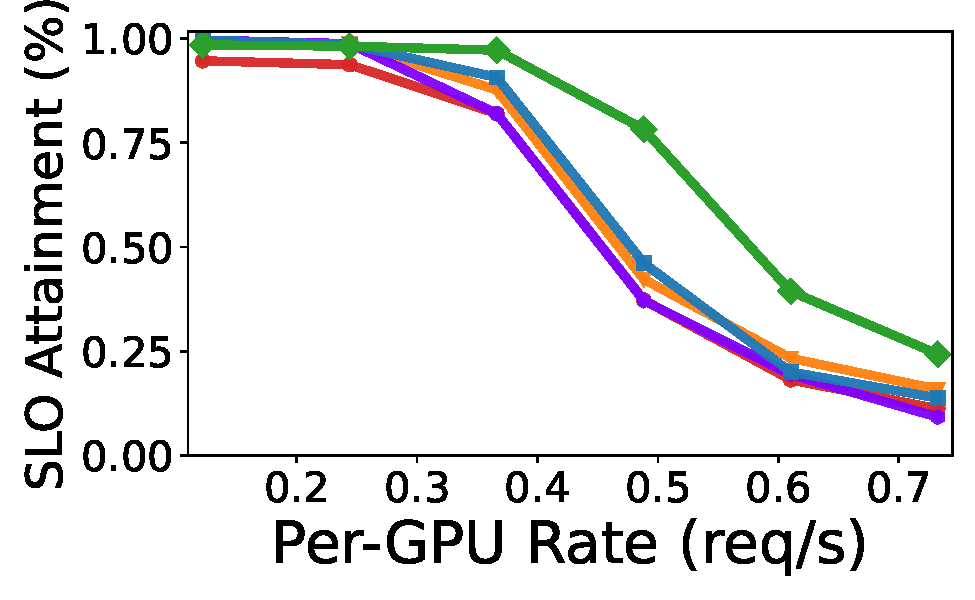
\includegraphics[width=\linewidth]{figures/evaluation/sim_qwenA/qwenA_coder_bw200.pdf}
        \caption{Qwen3-Coder}
        \label{fig:evaluation:qwenA:qwencoder_200}
    \end{subfigure}
    \hfill
    \begin{subfigure}[b]{0.24\linewidth}
        \centering
        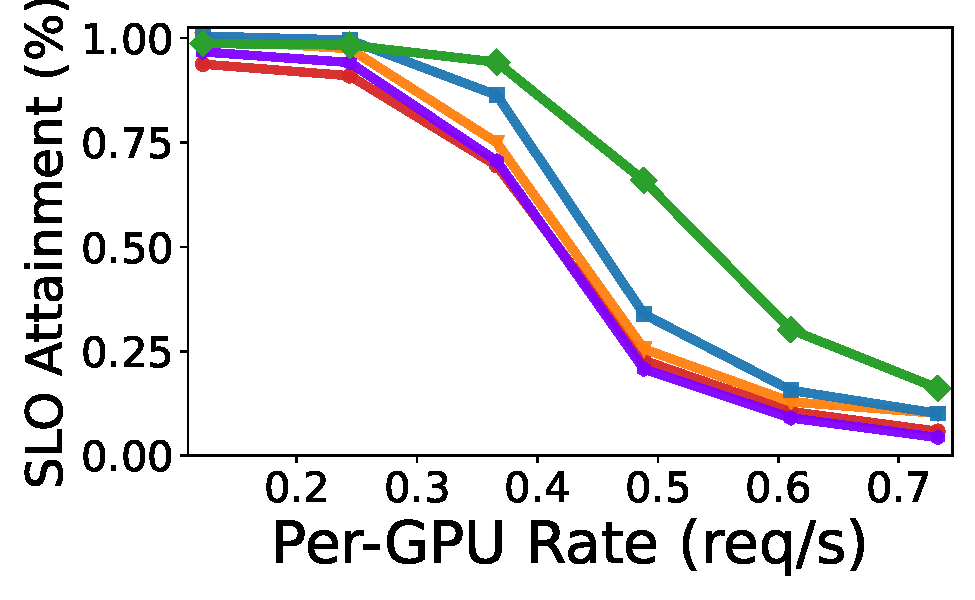
\includegraphics[width=\linewidth]{figures/evaluation/sim_qwenA/qwenA_grok2_bw200.pdf}
        \caption{Grok2}
        \label{fig:evaluation:qwenA:grok2_200}
    \end{subfigure}
    \caption{[Simulation] Performance on conversation workload (QwenA)
    }
    \label{fig:evaluation:qwenA}
\end{figure*}
